\documentclass[12pt]{extarticle}

\usepackage{graphicx}
\usepackage[utf8]{inputenc}
\usepackage[english,russian]{babel}
\usepackage[pdftex,unicode]{hyperref}
\usepackage[margin=15mm,left=2cm]{geometry}
\usepackage{indentfirst}
\usepackage{amsbib}
\usepackage{amsmath}
\usepackage{latexsym}

\sloppy
\clubpenalty=999
\widowpenalty=9999

\newtheorem{theorem}{Теорема}[section]
\newtheorem{lemma}[theorem]{Лемма}
\newtheorem{proposition}[theorem]{Утверждение}
\newtheorem{corollary}[theorem]{Следствие}

\newenvironment{proof}[1][Доказательство.]{\begin{trivlist}
\item[\hskip \labelsep {\bfseries #1}]}{\end{trivlist}}
\newenvironment{definition}[1][Определение.]{\begin{trivlist}
\item[\hskip \labelsep {\bfseries #1}]}{\end{trivlist}}
\newenvironment{example}[1][Example]{\begin{trivlist}
\item[\hskip \labelsep {\bfseries #1}]}{\end{trivlist}}
\newenvironment{remark}[1][Замечание]{\begin{trivlist}
\item[\hskip \labelsep {\bfseries #1}]}{\end{trivlist}}

\newcommand{\qed}{\nobreak \ifvmode \relax \else
      \ifdim\lastskip<1.5em \hskip-\lastskip
            \hskip1.5em plus0em minus0.5em \fi \nobreak
                  \vrule height0.75em width0.5em depth0.25em\fi}

% This is all for formatting and making the Table of Contents according to 
% spec. Don't play with it.
\makeatletter
\renewcommand\l@section[2]{%
    \ifnum \c@tocdepth >\z@
        \addpenalty\@secpenalty
        \addvspace{1.0em \@plus\p@}%
        \setlength\@tempdima{1.5em}%
        \begingroup
        \parindent \z@ \rightskip \@pnumwidth
        \parfillskip -\@pnumwidth
        \leavevmode \bfseries
        \advance\leftskip\@tempdima
        \hskip -\leftskip
#1\nobreak\ 
        \leaders\hbox{$\m@th\mkern \@dotsep mu\hbox{.}\mkern \@dotsep mu$}
    \hfil \nobreak\hb@xt@\@pnumwidth{\hss #2}\par
        \endgroup
    \fi}
\makeatother

\title{Критерий планарности для класса предикатных схем}
\author{Василевская И.\,Ю.}
\date{\today}

\begin{document}
    \begin{titlepage}
        \begin{center}
            Московский Государственный Университет им. М.В. Ломоносова\\
            Факультет Вычислительной Математики и Кибернетики\\
            Кафедра Математической Кибернетики\\
            магистратура, отделение <<МММ СБИС>>\\[6cm]

            \large {Василевская Инесса Юрьевна}\\
            \LARGE \textbf {Критерий планарности для класса предикатных схем}\\[0.8cm]
            \large \emph {Магистерская диссертация}\\[5.0cm]

            \begin{flushright}
                \large
                \begin{minipage}{0.40\textwidth}
                    \begin{flushleft}
                        \emph{Научный руководитель:}\\к.ф.м.н М.\,С.~Шуплецов
                    \end{flushleft}
                \end{minipage}
            \end{flushright}

            \vfill
            Москва\\
			2013
        \end{center}
    \end{titlepage}

\setcounter{page}{2}

\section*{Аннотация}
\label{anno}
В работе исследуется специальный класс дискретных управляющих систем~--- класс планарных предикатных схем, 
представляющий собой модификацию модели схем из предикатных элементов, в которой рассматриваются схемы,
граф которых является планарным, а входы расположены на внешней грани.
По аналогии с моделью СФЭ для полного базиса данной модели формулируется критерий планарной
реализуемости; описывается алгоритм преобразования произвольной непланарной предикатной схемы 
в заданном базисе в планарную предикатную схему и приводятся оценки сложности ``планаризации''.
\tableofcontents
\clearpage

\section{Введение}
\label{beginning}
Одной из основных задач математической кибернетики является задача синтеза управляющих систем.
Возникнув на рубеже 30-40 годов 20 века на основе ряда задач, связанных с логическим описанием и проектированием 
различных типов дискретных вычислительных устройств, задача синтеза обрела строгую математическую постановку в работах
Клода Шеннона (\cite{Shannon},~\cite{Shannon2}).

В общем виде задача синтеза рассматривается для какого-либо класса дискретных управляющих систем, 
наделенных определенной структурой
и характеризующихся поведением (функционированием) дискретного типа. 
При этом, обычно, структура схемы описывается графом специального
вида, а её функционирование~-- системой булевых функций, реализуемых
данной схемой. Предполагается, что структура схемы однозначно определяет ее функционирование и
рассматриваемый класс схем является полным, то есть схемами из данного класса можно реализовать любую булеву
функцию.

Среди класса дискретных управляющих систем условно можно выделить модели двух типов~-- функциональные и проводящие. 
Характерной чертой управляющих систем функционального типа является такой способ
функционирования, при котором значения реализуемых функций находятся как
решение некоторой системы (булевых) уравнений. В качестве примера моделей функционального типа
можно привести СФЭ. 
Модели проводящего типа характеризуются тем, что их 
функционирование определяется наличием или отсутствием проводимости между
входными и выходными полюсами при различных фиксированных значениях управляющих переменных. Яркими представителями 
этого класса являются двоичные решающие диаграммы или контактные схемы.

По аналогии с работой \cite{Shu11}, предикатные схемы можно представить как отдельный, предикатный, 
тип дискретных управляющих систем.
Основу для появления моделей предикатного типа заложила работа \cite{Bodnar4uk_f},
где рассматривалась операция суперпозиции и вопросы полноты для предикатов. 
Для моделей предикатного типа в работе \cite{graph_first} была предложена схемная интерпретация
в виде двудольного графа специальной структуры.

Модели предикатного типа применяются в различных областях науки, так как существенное количество задач 
можно естественно переформулировать в терминах множества объектов, связей между ними и набора ограничений, которым
должно удовлетворять решение. Схемы предикатного типа можно встретить в таких дисциплинах, как теория игр \cite{gt}, 
теория мультиагентных систем (\cite{mas}), математическая логика (\cite{ml}) и других. 
Особо следует отметить то, что модели предикатного типа можно эффективно применять для 
решения задач анализа и синтеза различных типов дискретных управляющих систем, 
включающих в себя как проводящие, так и функциональные элементы.  

Современное проектирование СБИС представляет собой многоуровневый процесс, на каждом из этапов которого
текущий вариант представления схемы должен удовлетворять большому количеству технологических ограничений. 
В качестве примера ограничений можно привести ограничение на число пересечений контактов на этапах размещения и трассировки.
Это делает актуальной задачу о минимизация числа реберных пересечений в графе схемы, а так же исследования
возможности ``планаризации'' произвольной схемы в заданном базисе. Для традиционного класса СФЭ критерий планарности
был установлен Яблонским \cite{yabl_planar}. В данной работе будет исследован аналогичный вопрос для класса предикатных схем.

\clearpage
\section{Описание модели}

Как было сказано во введении, предикатную модель можно представить в виде набора входных переменных,
которые принимают значения в домене $[0, 1]$, набора внутренних переменных, 
обеспечивающих связь между предикатными элементами, и набора ограничений~-- множества
предикатных элементов, определенного на каком-то подмножестве входных переменных модели, 
с заданной областью допустимых значений.
Решение задачи можно представить как множество таких наборов входных переменных, при которых все внутренние
переменные модели удовлетворяют набору ограничений.

Дадим определение предикатной схемы и ее функционирования по аналогии с \cite{Shu11}.

\begin{definition}
\label{pred_def}
\textit{Схемой из предикатных элементов} или \textit{предикатной схемой в базисе $\Pi$} назовем помеченный
неориентированный двудольный граф следующей структуры:

\begin{itemize}
\item каждая вершина из первой доли помечена некоторым множеством символов из алфавита X и/или 
множеством символов из алфавита Y. 
Алфавит $X$ соответствует \textit{входным} переменным предиката, а $Y$ ~-- его внутренним переменным, 
т.е. переменным, возникающим непосредственно в процессе вычисления; 

\item каждая вершина второй доли помечена некоторым символом $\pi_i$ из множества $\Pi$ и 
соединена $k$ ребрами, пронумерованными числами $1, \dots, k$, с вершинами из первой доли.
\end{itemize}
\end{definition}

Вершины из первой доли будем называть узлами схемы, а вершины из второй доли ~-- её предикатными элементами. 
Узлы схемы, соединенные ребрами с предикатным элементом, будем называть полюсами этого элемента, 
а узлы, соответствующие входным переменным, ~-- полюсами схемы.
При этом считается, что узел является $j$-м полюсом предикатного элемента и соответствует 
его $j$-ой переменной, если соединяющее их ребро имеет номер $j$. Полюс схемы, которому приписано 
более одной входной переменной, называется кратным полюсом этой схемы. 

Будем считать элементарной такую предикатную схему, которая состоит либо из изолированной полюсной вершины, 
либо только из одного предикатного элемента $\pi_i$, $1 < i < k$, где $k$ ~-- число полюсов указанного элемента.

Функционирование предикатной схемы на конкретном наборе определяется допустимостью состояния схемы на этом наборе.
Предикатная схема $\Sigma$ находится в допустимом состоянии на 
заданном наборе значений её полюсных переменных тогда и только тогда, 
когда существует такой набор значений внутренних переменных схемы, на котором все предикатные элементы схемы находятся в допустимых состояниях. 
Если же указанного набора значений внутренних переменных не существует, то считается, что схема находится в недопустимом состоянии на 
заданном наборе значений её полюсных переменных.

Предполагается, что предикатная схема $\Sigma$ реализует предикат $\pi$ от её полюсных переменных, 
если множество допустимых наборов $\pi$ 
совпадает с множеством тех наборов, на которых $\Sigma$ находится в допустимом состоянии. 
При этом схемы будем называть эквивалентными, если они реализуют равные предикаты. 

Отметим, что элементарная предикатная схема, состоящая из изолированной полюсной вершины, 
реализует тождественно истинный предикат.
 Будем считать также, что тождественно истинный (соответственно тождественно ложный)
 предикат реализуется любой предикатной схемой без входных полюсов, 
которая имеет непустое (соответственно пустое) множество допустимых состояний.

В общем случае граф предикатной схемы может содержать несколько компонент связности. 
В дальнейшем, будем считать, что схема не содержит компонент связности,
которые не имеют полюсных узлов и для которых существует хотя бы один допустимый набор, 
так как такие компоненты не влияют на функционирование схемы.

\subsection{Способы описания предикатных схем}
Существуют различные способы представления предикатных схем, каждый из которых лучше отражает определенные свойства данной 
модели. Так, например, предикатные элементы и отдельные взаимосвязи между ними, отображенные в графовой модели,
весьма наглядно отражают топологию схемы, в то время как для функционального описания схемы в смысле 
определения множества допустимых значений 
всей схемы или отдельных ее подсхем, естественно использовать такой способ описания функционирования предиката,
как выражение его области допустимых значений через характеристические функции. 
Отдельно стоит упомянуть и универсальную модель обобщенных задач выполнимости.

\subsubsection*{Графовое представление}

Нетрудно видеть из общего определения $\ref{pred_def}$ модели,
что представление предикатной схемы в виде помеченного неориентированного графа 
наглядно описывает топологию схемы и взаимосвязи 
между отдельными подсхемами.

В тех случаях, когда это не вызывает разночтений, не будем различать узел схемы и переменную, 
символ которой приписан данной вершине, а также предикатный элемент и сам предикат, отвечающий этому элементу. 
Также, для удобства, в некоторых случаях будем использовать упрощенное описание предикатной схемы, 
опуская пометки дуг и некоторых внутренних вершин.  

\subsubsection*{Модель характеристических функций}

Для представления допустимых наборов значений результирующей схемы или отдельных предикатных элементов, 
удобно использовать характеристические
функции. Так, функционирование предикатного элемента $\pi(x_1, \dots, x_k)$ с $k$ полюсами,
задается его характеристической функцией $\chi_{\pi}$ от $k$ переменных, 
связанных с указанными полюсами, и определяется тем, что предикатный элемент находится в допустимом состоянии на тех и 
только тех наборах значений этих переменных, на которых данная функция равна 1. 

В дальнейшем, предикат $\pi$, зависящий от $n$ переменных, будем обозначать $\pi(x_1, \dots, x_n)$, а 
$\Pi(x_1, \dots, x_n)$ будет соответствовать множеству кортежей (наборов значений, множеству истинности) 
предиката $\pi(x_1, \dots, x_n)$: $\Pi(x_1, \dots, x_n) = \{ \alpha | \chi_{\pi}(\alpha) = 1 \}$.

\subsubsection*{Модель обобщенных задач выполнимости}

\begin{definition}
Обобщенная задача выполнимости (CSP)\footnote{Constraint Satisfaction Problem}~--- это тройка $<V,D,C>$, где $V$~--- набор переменных, $D$~--- область определения (домен допустимых значений), 
а $C$~-- набор ограничений. Ограничения имеют вид $<t, R_n>$, где $t$~--- кортеж из $n$ переменных множества $V$, 
$R_n$~--- заданное на $D$ отношение арности $n$. 
Решением задачи CSP является набор значений переменных $V$, который удовлетворяет всем ограничениям из $C$. 
\end{definition}

Так, например, задачу 3-ВЫП можно рассматривать как обобщенную задачу выполнимости над булевым доменом, множество
ограничений $C$ которой состоит исключительно из зависящих от трех переменных отношений-конъюнкций.

В ряде работ рассматривалась вычислительная сложность задачи CSP. Несмотря на то, что в общем случае задача CSP
принадлежит классу NP, при введении определенных ограничений на множество $C$ или структуру так называемого
графа ограничений\footnote{constraints graph} существуют быстрые алгоритмы нахождения решения. 
Так, например, в \cite{Shaeffer78} показано, 
что, в тех случаях, когда множество $C$ представляет собой дерево, существуют полиномиальные алгоритмы нахождения решения.

Свести задачу определения функционирования предикатной схемы к нескольким задачам CSP можно следующим образом.

Пусть предикатная схема $\Sigma$ имеет $m$ входных переменных $x_1, \ldots , x_m$, 
$k$ внутренних переменных $y_1, \ldots , y_k$ и $n$ предикатных элементов $B = \pi_1, \dots , \pi_n$. 
Тогда, для определения функционирования этой схемы нужно найти допустимые значения внутренних переменных на всех $2^{m}$
наборах входных переменных. 

Нетрудно видеть, что эта задача может быть сведена к $2^m$ задачам CSP $<V, D, C>$ следующим образом:
$V$ = $Y$, $D = [0, 1]$, $C = B$. Перед началом вычисления каждой из задач, переменные $x_1, \ldots , x_m$ 
во всех ограничениях, их содержащих, отождествляются с соответствующими константами $\alpha_1, \ldots , \alpha_m$.

В данной работе в основном будут использоваться первые две модели, однако стоит отметить, что представление предикатных
схем с помощью обобщенных задач выполнимости позволяет использовать ранее полученные для CSP результаты для 
выяснения таких вопросов, как, например, сложность определения функционирования заданной схемы.

\subsection{Операции над предикатными элементами}

\begin{definition}
Суперпозицией двух предикатных схем, не имеющих общих вершин и пометок, 
будем называть их объединение с возможным отождествлением группы полюсов этих схем, 
которое сопровождается приписыванием новой (``объединенной'') вершине либо 
некоторого подмножества переменных данной группы, либо ``новой'' внутренней переменной.
\end{definition}

Выше были описаны две модели для представления предикатных схем: графовая, удобная для отображения топологии схемы; 
и характеристических функций, подходящая для работы с множеством допустимых значений отдельных элементов схемы. Далее 
будут рассмотрены частные случаи операции суперпозиции и их отображение на каждую из моделей.

Отметим, что для описания функционирования предикатных схем в ряде статей (\cite{Marchenkov}, \cite{Zhuk}, \cite{Shu09})
использовались $(\exists, \&)$~-формулы, а операция суперпозиции двух предикатов $\pi_1$ и $\pi_2$ соответствовала
операции конъюнкции.

\begin{definition}
Конъюнкцией $\pi_1(x_1, \dots, x_m)$ и $\pi_2(x_1, \dots, x_n)$ называется такой $(m+n)$-местный предикат $\pi$, что
$$\pi(x_1, \dots, x_m, x_{m+1}, \dots, x_{m+n}) = \pi_1(x_1, \dots, x_m) \& \pi_2(x_{m+1}, \dots, x_{m+n})$$.
\end{definition}

Заметим, что если у предикатов, к которым применяется операция конъюнкции,
не будет общих переменных, то множество кортежей $\Pi$ результирующего предиката 
$\pi$ представляет собой декартово произведение множества кортежей предиката $\pi_1$ и $\pi_2$ соответственно:
$\Pi = \Pi_1 \otimes \Pi_2$.

На рисунках, иллюстрирующих операции, вершины, закрашенные белым цветом, соответствуют входным переменным предиката; 
вершины, закрашенные черным цветом~-- внутренним переменным, причем, если вершина, закрашенная черным цветом, 
не помечена никакой переменной, то считается, что к предикату была применена операции 
проекции по данной переменной (пометка будет отсутствовать только если проецируемую переменную можно однозначно определить).
Множество кортежей, перечисленных в предикатной вершине, является множеством определения данного предиката. 
Предикатная схема, расположенная слева от стрелки, иллюстрирует графовое представление результата применения той или иной
операции; предикат, расположенный справа соответствует результирующему предикату $\pi$ после применения операции 
в модели характеристических функций.

Частными случаями операции суперпозиции являются перечисленные ниже операции.

\label{operations}
\begin{itemize}
    \item Проекция или снятие полюсной переменной схемы
    
    С точки зрения графовой модели, операция проекции предиката $\pi_1(x_1, \dots, x_n)$ по переменной $x_i$
    заключается в снятии пометки переменной $x_i$ со всех вершин, ранее ею помеченных.

    C точки зрения модели характеристических функций,
    по аналогии с \cite{Marchenkov}, проекцией предиката $\pi_1(x_1, \dots, x_n)$ по переменной $x_i$ называется такой
    $(n-1)$-местный предикат $\pi$, что:
    $\pi(x_1, \dots, x_{i-1}, x_{i+1}, \dots, x_n) = (\exists x_i) \pi_1(x_1, \dots, x_{i-1}, x_i, x_{i+1}, \dots, x_n)$.

    \begin{figure}[htb]
    \centering
    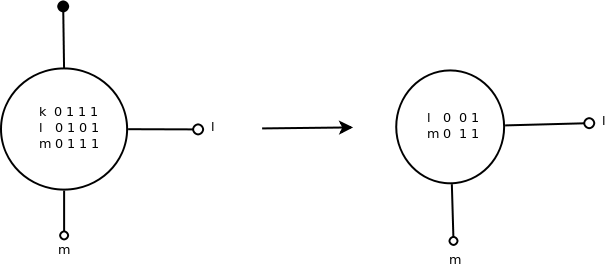
\includegraphics[width=0.7\textwidth]{project_op.png}
    \caption{Операция проекции}
    \label{fig:project_op}
    \end{figure}

    \samepage
    \item Суперпозиция с отождествлением полюсов

    С точки зрения графовой модели, в результате суперпозиции предикатов с отождествлением по k переменным, каждая пара
    отождествляемых вершин заменяется одной, которой приписываются пометки отождествляемых вершин обоих предикатов.

    С точки зрения модели характеристических функций, 
    суперпозицией $\pi_1(x_1, \dots, x_m)$ и $\pi_2(y_1, \dots, y_n)$ с отождествлением по первым k переменным 
    называется $(m+n)$-местный предикат
    $\pi(x_1, \dots, x_k, x_{k+1}, \dots, x_m, y_{m+1}, \dots, y_n) = \pi_1(x_1, \dots, x_k, x_{k+1} \dots, x_m) \& \pi_2(x_1, \dots, x_k, y_{k+1}, \dots, y_n)$.

    \begin{figure}[htb]
    \centering
    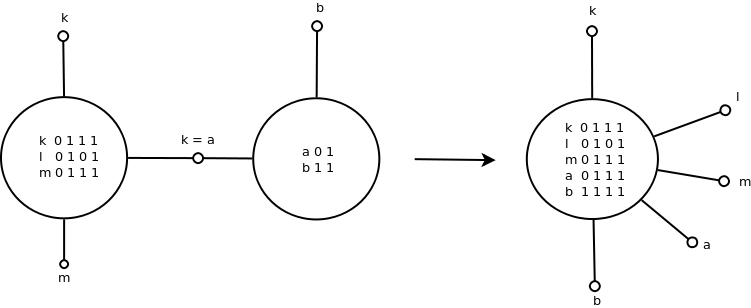
\includegraphics[width=0.9\textwidth]{join_op.png}
    \caption{Операция суперпозиции с отождествлением}
    \label{fig:join_op}
    \samepage
    \end{figure}

    Отдельно стоит выделить операцию суперпозиции предикатов с отождествлением не более чем по 2 переменным с
    ограничением на дальнейшее использование внутренних переменных результирующего предиката: внутренняя переменная
    может быть использована в последующих операциях суперпозиции тогда и только тогда, когда это не приведет
    к реберным пересечениям или перемещению входных переменных предиката на внутренюю грань. В дальнейшем такую операцию
    будем называть ограниченной суперпозицией с отождествлением по 2 переменным.
    
    \item Отождествление входов схемы
    
    Отождествление входов схемы можно рассматривать как частный случай операции суперпозиции с отождествлением, в 
    которой участвует не пара предикатов $\pi_1(x_1, \dots, x_n)$ и $\pi_2(x_1, \dots, x_m)$, а один предикат 
    $\pi_1(x_1, \dots, x_n)$.

    \begin{figure}[htb]
    \centering
    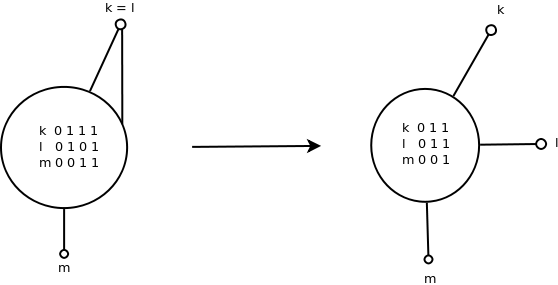
\includegraphics[width=0.7\textwidth]{join_ins_op.png}
    \caption{Операция отождествления входов}
    \label{fig:join_ins_op}
    \samepage
    \end{figure}

    \item Подстановка констант $(\sigma_1, \dots, \sigma_k)$ вместо первых k переменных

    Будем называть предикатами-константами предикаты $\pi_0(x)$ и $\pi_1(x)$, множества определения которых состоят
    из соответствующей константы: $\Pi_0=\{ (0) \}, \Pi_1=\{ (1) \}$.

    В таком случае, операцию подстановки констант вместо k переменных предиката $\pi'(x_1, \dots, x_n)$ 
    можно определить как операцию суперпозиции предиката $\pi'(x_1, \dots, x_n)$ и k предикатов 
    $\pi_{\sigma}(x)$, где $\sigma \in [0,1]$, и каждый из предикатов-констант отождествляется с предикатом $\pi'$ по
    по переменной $x$.

    В модели характеристических функций данное преобразование будет выглядеть следующим образом:
    $\pi(x_1, \dots, x_n) = \pi'(\sigma_1, \dots, \sigma_k, x_{k+1}, \dots, x_n)$. 
    
    \begin{figure}[htb]
    \centering
    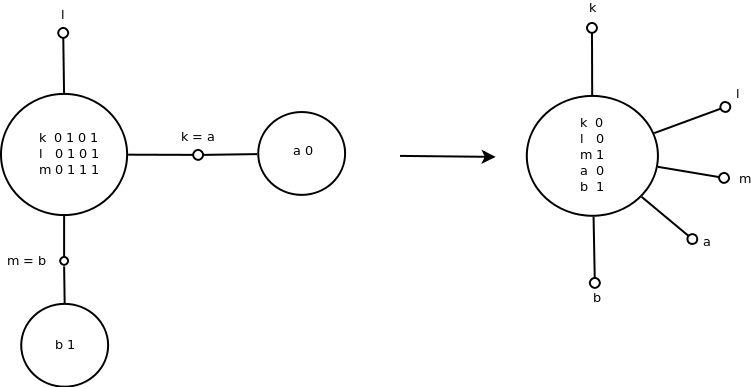
\includegraphics[width=0.8\textwidth]{join_const_op.png}
    \caption{Операция подстановки констант}
    \label{fig:join_const_op}
    \samepage
    \end{figure}

    \item Отрицание переменной

    Рассмотрим предикат $\pi_{\neg}(x_1, x_2)$, множество определения которого имеет вид $\Pi_{\neg} = \{ (01), (10) \}$.
    Тогда операцию отрицания переменной $x_i$ можно представить как суперпозицию исходного предиката и предиката $\pi_{\neg}$
    с отождествлением по переменной $x_i$.
    
    В модели характеристических функций это преобразование будет выглядеть следующим образом:
    $\pi(x_1, \dots, y, \dots, x_k) = \pi_1(x_1, \dots, x_i, \dots, x_k) \& \pi_{\neg}(x_i, x_2)$.

    Заметим, что для того, чтобы в результирующий предикат $i$-ая переменная входила только с отрицанием, следует сделать 
    проекцию по переменной $x_i$. Иначе в кортежах результирующего предиката найдутся 2 координаты, значения которых
    для всех наборов будут противоположными (на рис. \ref{fig:join_neg_op} им соответствуют переменные b и k).

    \begin{figure}[htb]
    \centering
    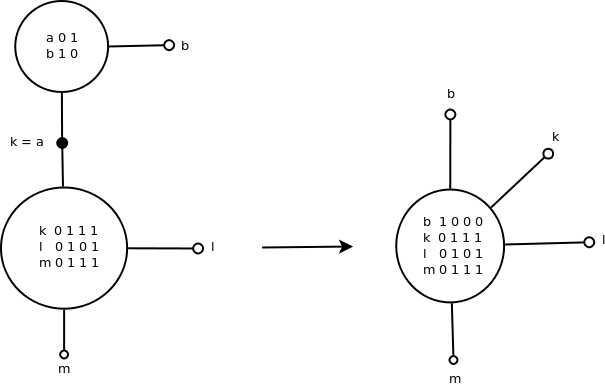
\includegraphics[width=0.8\textwidth]{join_neg_op.png}
    \caption{Операция отрицания переменной}
    \label{fig:join_neg_op}
    \samepage
    \end{figure}

\end{itemize}
\subsection{Полнота}

\begin{definition}
Система предикатов $B = \{ \pi_1, \dots, \pi_k \}$ является полной, если, 
применением операций суперпозиции к предикатам из B, можно получить 
предикат $\pi(x_1, \dots, x_n)$ с произвольной характеристической 
функцией $\chi_{\pi} \in P_2^n$, где $P_2^n$ есть множество всех булевых функций от n переменных.
\end{definition}

\begin{definition} ФАЛ
$f (x_1, \ldots, x_n)$ от $n$ переменных сохраняет предикат $ (x_1, \ldots, x_m)$ от $m$
переменных тогда и только тогда, когда для любых $n$ допустимых наборов $\alpha^i = (\alpha_1^i, \ldots, \alpha_n^i), 
i = \overline{1, n}$ значений переменных предиката $\pi$ набор
значений $( f(\alpha_1^1, \ldots, \alpha_1^n), \ldots, f(\alpha_m^1, \ldots, \alpha_m^n) )$
тоже является допустимым для предиката $\pi$.
\end{definition}

Определим следующие классы предикатов:
\begin{itemize}
    \item{$T_0$}~-- множество всех предикатов, сохраняющих константную ФАЛ 0;
    \item{$T_1$}~-- множество всех предикатов, сохраняющих константную ФАЛ 1;
    \item{S}~-- множество всех предикатов, сохраняющих ФАЛ $\bar{x}$;
    \item{K}~-- множество всех предикатов, сохраняющих все конъюнкции от двух и более переменных;
    \item{D}~-- множество всех предикатов, сохраняющих все дизъюнкции от двух и более переменных;
    \item{SM}~-- множество всех предикатов, сохраняющих все монотонные самодвойственные ФАЛ;
    \item{SL}~-- множество всех предикатов, сохраняющих все монотонные линейные ФАЛ.
\end{itemize}

\begin{theorem}
\label{Post}
\textbf{(Критерий полноты для предикатных схем)}. Система из $B$ предикатов является полной $\iff$
она не лежит целиком ни в одном из 7 предполных классов: $T_0, T_1, SM, SL, S, K, D$. \cite{Shu11} 
\end{theorem}

\begin{definition}
Шефферовым базисом будем называть полный базис, состоящий из одного предиката. Сам этот предикат
будем называть шефферовым предикатом.
\end{definition}


\begin{definition}
Будем говорить, что предикат $\pi_1$ входит в предикат $\pi_2$, или что предикат $\pi_2$ является
расширением предиката $\pi_1$, если множество кортежей $\Pi_1$ предиката $\pi_1$ 
содержится во множестве кортежей $\Pi_2$ предиката $\pi_2$.
\end{definition}

\begin{definition}
Набор $(\alpha_1, \dots, \alpha_n)$ называется существенным для предиката $\pi$ арности $n$, если
$\pi(\alpha_1, \dots, \alpha_n) = 0$ и существует $b_1, \dots, b_n$ такие, что для любого $i \in \{ 1, 2, \dots, n\}$
выполняется 
$\pi(\alpha_1, \dots, \alpha_{i-1}, b_i, a_{i+1}, \dots, a_n)$ = 1.
\end{definition}

\begin{definition}
Предикат арности $n$ называется существенным, если он не может быть представлен в виде конъюнкции
предикатов меньшей арности.
\end{definition}

\begin{lemma}
\label{susch_lemma}
Следующие три условия эквиваленты: 
\begin{enumerate}
\item предикат $\pi$ является существенным;
\item $\pi \neq \pi_{\neg}(x_1, x_2)$, где $\Pi_{\neg} = \{ (01), (10) \}$;
\item для предиката $\pi$ существует существенный набор. \cite{Zhuk}
\end{enumerate}
\end{lemma}

\clearpage

\section{Постановка задачи}
Необходимо рассмотреть модифицированную модель предикатных схем~-- модель планарных предикатных схем, 
отличие которой от обычной модели состоит в наложении особых ограничений на граф схемы и набор допустимых операций 
суперпозиции. 

Определения полноты вводятся по аналогии с обычной моделью предикатных схем. Так, например, полный базис
в модели планарных предикатных схем есть такая система предикатов, что 
применяя набор допустимых
операций над элементами системы, можно получить планарную схемную реализацию предиката $\pi$, множество
допустимых наборов которого задается соответствующей произвольной характеристической функцией $\chi_{\pi} \in P_2^n$. 

Для описанной выше модели требуется сформулировать и обосновать критерий ``планарной реализуемости'', привести и оценить алгоритм
преобразования произвольной непланарной схемы в заданном базисе.
\clearpage

\section{Обоснование планарности}

\begin{definition}
Предикатная схема, которую можно уложить на плоскости без реберных пересечений таким образом, что полюса предикатов, 
соответствующие внешним переменным, лежат на внешней границе, называется планарной. 
\end{definition}

\begin{definition}
Базис называется планарным, если в нем можно реализовать любой предикат планарной схемой.
\end{definition}

\begin{definition}
Операции над предикатной схемой, сохраняющие планарность схемы, будем называть операциями планарной суперпозиции.
\end{definition}

\begin{lemma}
\label{lemma_planar_ops}
Ограниченная суперпозиция с отождествлением по двум переменным, проекция,
подстановка констант, отождествление входов и отрицание переменной являются операциями планарной суперпозиции.
\end{lemma}
\begin{proof}
Из определения операций над предикатами в \S \ref{operations} следует, что операция проекции, операция подстановки
констант вместо k переменных, отождествления входов и отрицания переменной не меняют планарность схемы. 
Действительно, при операции проекции, граф предикатной схемы остается неизменным; 
при операции отождествления входов количество вершин-переменных уменьшается на 1, число же ребер остается прежним, 
однако появляется дуга от предикатного элемента до отождествляемого входа;
в случае подстановки констант добавляется k вершин, соответствующих предикатным элементам
и k ребер, что не может добавить к графу схемы даже новых циклов;
отрицание переменной добавляет к графу простую цепь. 

Ограниченная суперпозиция с отождествлением по 2 переменным не влияет на планарность в силу наложенных на
нее ограничений, 
$\Box$.
\end{proof}

Покажем, что, применяя к предикатам $\pi_S, \pi_K, \pi_D$ только следующие операции планарной суперпозиции ~-- проекцию,
суперпозиции с отождествлением не более чем по 2 переменным и отождествления входов, 
можно получить предикаты-константы
$\pi_0(x_1), \Pi_0=\{ (0) \}$ и $\pi_1(x_1), \Pi_1=\{ (1) \}$ и предикат-отрицание 
$\pi_{\neg}(x_1, x_2), \Pi_{\neg}=\{ (01), (10) \}$.

\subsection{Получение констант}
\begin{lemma}
\label{eq:const}
Из предиката $\pi_S \notin S$, где $S$~-- класс предикатов, сохраняющих $\bar{x}$, 
применением операции отождествления входов и подстановки констант,
можно получить планарную реализацию предикатов-констант $\pi_0(x), \pi_1(x)$.
\end{lemma}

\begin{proof}
Так как $\pi_S \notin S$, то в $\Pi_S$ существуют такой набор
$\alpha_1$, что его отрицание не принадлежит множеству определения предиката:
$\exists \alpha_1 \in \Pi_S, \bar{\alpha_1} \notin \Pi_S$.
Применяя операцию отождествления входов к тем переменным, которые равны $\sigma$ на наборе $\alpha$,
получаем один из предикатов-констант $\pi_{\sigma}(x)$.

Если $\sigma = 0$, то рассмотрим предикат 
$\pi_{T_0}(x_1, \dots, x_n) \notin T_0$. Очевидно, что этот предикат не содержит нулевой набор. 
Проецируем по $(n-2)$ переменным таким образом, чтобы 
$\pi'(x_1, x_2) = \exists {x_{i_1}, \dots, x_{i_{n-2}}} \pi_{T_0}(x_1, x_2, x_{i_1}, \dots, x_{i_{n-2}})$
имел в качества множества наборов $\Pi' = { (01) }$ или всевозможные расширения, не содержащие набор $(00)$.
Далее, подставляя вместо одной из переменных 0, получаем предикат $\pi_1(x)$, $\Box$. 

В случае константы 1, поступаем аналогично. 
Заметим, что при получении константы использовались только операции планарной суперпозиции, следовательно, 
результирующие предикаты-константы планарны, $\Box$.
\end{proof}
\begin{figure}[htb]
\centering
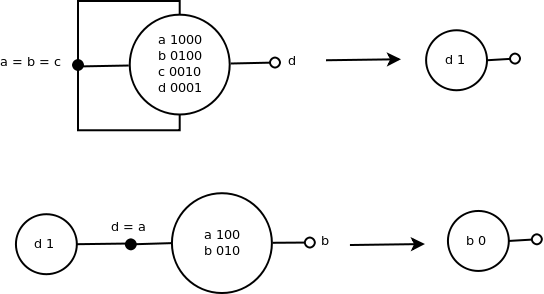
\includegraphics[width=0.6\textwidth]{const.png}
\caption{Получение константы}
\label{fig:constant}
\end{figure}

\subsection{Получение отрицания}
\begin{lemma}
\label{eq:negate}
Пусть даны предикаты $\pi_K \notin K, \pi_D \notin D$, где $K (D)$~-- класс предикатов, 
сохраняющих конъюнкции (дизъюнкцию) двух и более переменных.
Тогда, применением операций подстановки констант и проекции
к предикатам $\pi_K, \pi_D$, можно получить планарную реализацию предиката $\pi_{\neg}$.
\end{lemma}

\begin{proof}
Вначале проведем доказательство для случая, когда оба предиката, $\pi_K$ и $\pi_D$ зависят от 2 переменных.

Так как $\pi_K \notin K$, то найдутся такие наборы $\alpha_1$ и $\alpha_2$ из области определения предиката $\Pi_K$, что
$\alpha_1\&\alpha_2=\beta, \beta \notin \Pi$, причем эти наборы должны отличаться как минимум по двум переменным $x_i, x_{j}$.
Значит, либо предикат $\pi_K(x_1, x_2)$ будет являться искомым предикатом $\pi_{\neg}$, либо его множество
допустимых значений будет иметь вид $\Pi_K = \{ (01), (10), (11) \}$. 
Проводя аналогичные рассуждения для $\pi_D$, получим, что либо $\pi_D(y_1, y_2) = \pi_{\neg}$, либо $\Pi_D = \{ (00), (01), (10) \}$.
Тогда, производя операцию ограниченной суперпозиции с отождествлением по переменным $x_1=y_1, x_2=y_2$, получаем
предикат $\pi_{\neg}$.

Пусть теперь один из предикатов зависит более чем от 2 переменных. Без ограничения общности, будем считать, что это $\pi_K$.
Так как $\pi_K \notin K$, то найдутся такие наборы $\alpha_1$ и $\alpha_2$ из области определения предиката $\Pi_K$, что
$\alpha_1\&\alpha_2=\beta, \beta \notin \Pi$, причем эти наборы должны отличаться как минимум по двум переменным $x_i, x_{j}$.
Выделим из множества переменных предиката подмножество $M = \{ x_t | t \neq i, t \neq j, \alpha_{1_t} \neq \alpha_{2_t} \}$ и 
подмножество $N = X \backslash \{ M \bigcup \{x_i, x_j\} \}$.
Во множество M входят переменные, соответствующие противоположным значениям координат наборов $\alpha_1$ и $\alpha_2$.
Произведя операцию проекции по этим переменным, а затем подставив соответствующие
константы вместо переменных из N, получим предикат $\pi_{\neg}$.
Заметим, что при получении константы использовались только операции планарной суперпозиции, следовательно, 
результирующие предикаты-константы планарны, $\Box$.
\end{proof}
\begin{figure}[htb]
\centering
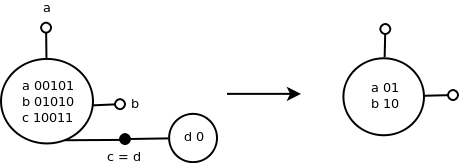
\includegraphics[width=0.6\textwidth]{negate.png}
\caption{Получение $\pi_{\neg}$}
\label{fig:negation}
\end{figure}


Из лемм \ref{lemma_planar_ops}, \ref{eq:const} и \ref{eq:negate} вытекает важное следствие:
\begin{corollary}
\label{can_use_ops}
Если $B$~-- полный предикатный базис по критерию полноты для предикатных схем
\ref{Post}, то к предикатам из B допустимо применение полного набора операций 
планарной суперпозиции, включая отрицание переменной и подстановку констант.
\end{corollary}

\subsection{Основные утверждения}
\label{planar_chapter}
\subsection{Планарные базисы}

\begin{figure}[htb]
\centering
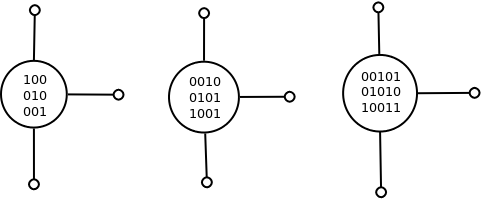
\includegraphics[width=0.6\textwidth]{scheff3.png}
\caption{Шефферовы предикаты от 3 переменных}
\label{fig:sheff}
\end{figure}

\label{planar_basis}

\begin{definition}
Минимальным предикатом $\pi_{min}(x_1, \dots, x_n) \notin P$, где $P$~-- один из предполных классов, будем называть такой 
предикат $\pi$, что $\forall i: \pi'(x_1, \dots, x_{n-1}) = \exists x_i \pi_{min}(x_1, \dots, x_{i}, \dots, x_n) \implies \pi' \in P$. 
Т.е. любой предикат,
полученный из $\pi_{min}$ проекцией по одной из переменных предиката, принадлежит $P$.
\end{definition}

\begin{definition}
Рассмотрим предикат 
$\pi$, множество кортежей которого имеет вид
\begin{center}
\begin{tabular}{ccc}
$(\alpha, \bar{\alpha}, \bar{\alpha}, \dots, \bar{\alpha}, \bar{\alpha})$\\
$(\bar{\alpha}, \alpha, \bar{\alpha}, \dots, \bar{\alpha}, \bar{\alpha})$\\
$\ldots$\\
$(\bar{\alpha}, \bar{\alpha}, \bar{\alpha}, \dots, \bar{\alpha}, \alpha)$
\end{tabular}
\end{center}

Нетрудно видеть, что $\pi$~-- существенный предикат, а
$(\bar{\alpha}, \bar{\alpha}, \dots, \bar{\alpha})$~-- существенный набор. 
В дальнейшем, предикаты, множество кортежей которых обладает такой структурой, будем называть 
симметричными предикатами порядка n и обозначать $\pi_{symm}^n$. Нетрудно видеть, что существенный предикат является 
расширением симметричного предиката, а характеристическая функция $\pi_{symm}^n$ представляет собой симметрическую функцию
с рабочим числом 1 или $(n-1)$.
\end{definition}

\begin{lemma}
\label{eq:planar_algo}
Существует алгоритм преобразования непланарной предикатной схемы $\Sigma$ в базисе $B=\{\pi_{symm}^3\}$
в планарную предикатную схему $\Sigma'$ в базисе B.
\end{lemma}
\begin{proof}
Так как в базисе $B=\{\pi_{symm}^3\}$ предикат 
$\pi_{linear}$, с множеством допустимых наборов $\Pi_{linear} = \{ (001), (010), (100), (111) \}$, 
можно реализовать планарной схемой (см. рис. \ref{fig:linear_3}, где вместо $+$ используется операция
отрицания суммы по модулю 2 ($\bar{\oplus}$)), то, замещая каждое реберное пересечение исходной схемы
на 3 предиката $\pi_{linear}$ по алгоритму на рис. \ref{fig:xor}, получаем планарную реализацию требуемого предиката
в базисе B, $\Box$.
\end{proof}

\begin{figure}[htb]
\centering
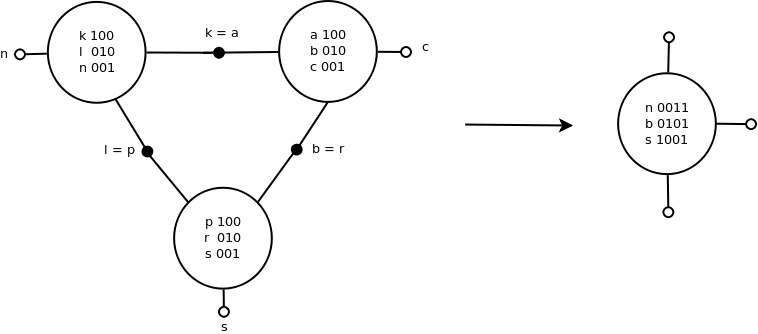
\includegraphics[width=0.8\textwidth]{linear.png}
\caption{Реализация $\pi_{linear}$ в базисе $B = \{ \pi_{symm}^3 \}$}
\label{fig:linear_3}
\end{figure}

\begin{figure}[htb]
\centering
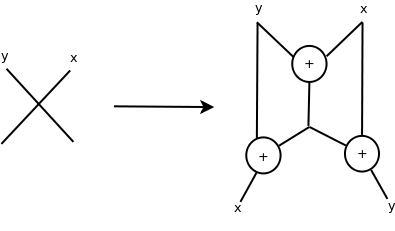
\includegraphics[width=0.5\textwidth]{intersection.png}
\caption{Получение планарной схемы}
\label{fig:xor}
\end{figure}

\begin{lemma}
\label{eq:lemma_sm}
Если $\pi \notin SM$, где $SM$~-- класс предикатов, сохраняющих все монотонные самодвойственные функции,
то, применяя операции проекции и отрицания переменной,
можно получить $\pi_{min} \notin SM$, причем $\pi_{min}$ будет являться расширением симметричного предиката.
\end{lemma}

\begin{proof}
Рассмотрим $\pi_{min} \notin SM$. Пусть $\widetilde{\beta} = (\beta_1, \dots, \beta_k)$~-- набор, полученный в результате
применения какой-то несамодвойственной функции, которую предикат не сохраняет.
Ясно, что $\widetilde{\beta} \notin \Pi_{min}$, т.е. $\widetilde{\beta} \neq \forall \widetilde{\alpha} \in \Pi_{min}$.
Однако, для соблюдения условия 
минимальности предиката, а именно присутствия свойства принадлежности классу $SM$, всеми предикатами, полученными
из $\pi_{min}$ проекцией по какой-либо переменной,
$\Pi_{min}$ должно содержать наборы 
$(\bar{\beta_1}, \beta_2, \dots, \beta_k), (\beta_1, \bar{\beta_2}, \dots, \beta_k), \dots, (\beta_1, \beta_2, \dots, \bar{\beta_k})$.

Нетрудно видеть, что набор $(\bar{\beta_1}, \bar{\beta_2}, \dots, \bar{\beta_k})$~-- существенный для $\pi_{min}$.

Так как класс $SM$ замкнут относительно операции отрицания переменной,
применяя эту операцию к $\pi_{min}$ можно получить $\pi'_{min}$,
такой, что набор $(\sigma, \sigma, \dots, \sigma)$ является для него существенным, а сам $\pi'_{min}$ является расширением 
симметричного предиката, $\Box$.
\end{proof}

\begin{corollary}
\label{lemma_sm_corollary} Из любого несамодвойственного предиката 
$\pi \notin SM $, применением операций планарной суперпозиции можно получить минимальный предикат $\pi_{min} \notin SM$,
который будет являться существенным предикатом с существенным набором
$ \alpha = (\sigma, \sigma, \dots, \sigma), \sigma \in \{0, 1\}$.
\end{corollary}

\begin{lemma}
\label{eq:super_new}
Пуcть $\pi \notin SM$, $\pi$~-- расширение симметричного предиката $\pi_{symm}^3$. 
Тогда, применяя операции планарной суперпозиции, можно получить планарную реализацию $\pi_{linear}$.
\end{lemma}

\begin{proof}
По условию, $\Pi = \Pi_{symm}^3 \bigcup A$, где
$ A \subseteq \{ (\alpha \bar{\alpha} \alpha), (\alpha \alpha \bar{\alpha}), (\bar{\alpha} \alpha \alpha), (\alpha \alpha \alpha) \} $.

Заметим, что во всех наборах из A от 2 до 3 координат равны $\alpha$, и $|A| = k, 1 \leq k \leq 4$.
Рассмотрим предикат $\pi_1(y_1, y_2)$ с множеством наборов 
$\Pi_1 = \{ (\bar{\alpha}, \bar{\alpha}), (\bar{\alpha}, \alpha), (\alpha, \bar{\alpha})\}$.

Примененяя операцию суперпозиции с отождествлением по 2 переменным $x_{i_1}=y_1, x_{i_2}=y_2$
исходного предиката $\pi(x_1, x_2, x_3)$ 
и предиката $\pi_1(y_1, y_2)$, 
где $i_1 \neq i_2 \neq j$,
\[ j = \left \{
  \begin{array}{l l}
     t & \quad \text{если $\exists \widetilde{\beta}=(\beta_1, \beta_2, \beta_3) \in A, \beta_t=\bar{\alpha}$ }\\
     \forall t \in [1, 3] & \quad \text{если $A = \{ (\alpha, \alpha, \alpha)\}$}
            \end{array} \right. \]
не более чем k раз, можно убрать ``лишние'' наборы и получить симметричный предикат.

Остается получить предикат $\pi_1(x_1, x_2)$.
Если $\pi_1(x_1, x_2)$ не получается из $\pi(x_1, x_2, x_3)$ проекцией по какой-либо переменной, то рассмотрим 2 случая. 

1. Пусть $A \neq \{ (\alpha, \alpha, \alpha) \}$. Тогда
$\exists \widetilde{\beta}=(\beta_1, \beta_2, \beta_3) \in A, \beta_t=\bar{\alpha}$. 
Подставив на место $t$-ой переменной
предиката $\pi$ константу $\bar{\alpha}$, и спроецировав по переменной t получим: 
предикат $\pi_1'(x_1, x_2)$ с множеством кортежей
$\Pi_1'=\{(\bar{\alpha}, \alpha), (\alpha, \bar{\alpha}), (\alpha, \alpha)\}$, из которого искомый предикат
$\pi_1$ получается применением операции отрицания 2 переменных.

В базисе из симметричного предиката $\pi_{symm}^3$ предикат $\pi_{linear}$ получается известным образом по лемме
\ref{eq:planar_algo}.

2. Пусть $A = \{ (\alpha, \alpha, \alpha) \}$. Тогда $\pi=\pi_{linear}, \Box$.
\end{proof}

Следующие две леммы показывают как, применяя операции планарной суперпозиции, от симметричного предиката
размерности n или его расширения, перейти к симметричному предикату размерности $(n-1)$ или его расширению.

\begin{lemma}
\label{eq:svedenie1}
Если $\pi(x_1, \dots, x_n) = \pi_{symm}^n, n > 3$, то, 
применяя операции подстановки констант и проекции, можно получить планарную реализацию $\pi_{symm}^{n-1}$.
\end{lemma}

\begin{proof}
Так как 
$\pi \notin SM$, то у предиката $\pi$ есть существенный набор $\widetilde{\alpha} = (\sigma, \dots, \sigma)$.
Тогда, производя операцию подстановки константы $\sigma$ вместо одной из переменный предиката, и последующую 
операцию проекции, получаем предикат $\pi_1(x_1, \dots, x_{n-1}) = \pi_{symm}^{n-1}, \Box$
\end{proof}

\begin{lemma}
\label{eq:svedenie2}
Если $\pi(x_1, \dots, x_n) \notin SM, n > 3$, то, применяя операции подстановки констант, отрицание переменных и 
проекции, можно получить планарную реализацию $\pi_1(x_1, \dots, x_{n-1}) \notin SM, \Box$.
\end{lemma}

\begin{proof}
По следствию \ref{lemma_sm_corollary}, применением операций планарной суперпозиции над $\pi$, можно получить 
$\pi_{min} \notin SM$ с существенным набором $\alpha=(\sigma, \dots, \sigma) \notin \Pi_{min}$. 
Далее, подставляя константу $\sigma$ вместо одной из переменных предиката $\pi_{min}$ и производя операцию проекции по
этой переменной, получаем предикат $\pi_1$, который
не принадлежит $SM$, и зависит от $n-1$ переменной, $\Box$.
\end{proof}

\section{Алгоритм планарного сведения}

\begin{theorem}
\label{Theo1}
Пусть дана непланарная предикатная схема $\Sigma$ в полном предикатном базисе $B$, максимальная
арность элементов которого равна 3.
Тогда из $\Sigma$, применением операций планарной суперпозиции, можно получить схему $\Sigma'$,
реализующую тот же предикат, что и $\Sigma$, но являющуюся планарной.
\end{theorem}
\begin{proof}
Приведем конструктивный алгоритм преобразования исходной схемы.

Вначале получаем планарную реализацию предикатов $\pi_0, \pi_1$ и $\pi_{\neg}$ 
по леммам \ref{eq:const} и \ref{eq:negate}. Их наличие, по лемме \ref{can_use_ops},
делает доступным весь набор операций планарной суперпозиции. 

Далее заменяем каждое реберное пересечение по лемме \ref{eq:planar_algo}. 

Полученная в результате вышеописанных преобразований схема является планарной, $\Box$.
\end{proof}

\begin{theorem}
\label{Theo2}
Пусть дана непланарная предикатная схема $\Sigma$ в полном предикатном базисе $B$. 
Тогда из $\Sigma$, применением операций планарной суперпозиции, можно получить схему $\Sigma'$,
реализующую тот же предикат, что и $\Sigma$, но являющуюсь планарной.
\end{theorem}

\begin{proof}
Предикаты $\pi_0, \pi_1, \pi_{\neg}$ получаем аналогично доказательству теоремы \ref{Theo1}.

Выделяем из базиса B $\pi(x_1, \dots, x_n) \notin SM$. По леммам \ref{eq:svedenie1} и \ref{eq:svedenie2}, 
применяя операции планарной суперпозиции к предикату $\pi(x_1, \dots, x_n)$, можно получить 
предикат $\pi'(x_1, x_2, x_3)$, являющийся либо симметричным предикатом от 3 переменных, либо его расширением. 

Далее, по лемме $\ref{eq:super_new}$ из предиката $\pi'$ получаем $\pi_{linear}$ и преобразовываем схему в планарную
по лемме \ref{eq:planar_algo}, $\Box$.
\end{proof}

Из теоремы \ref{Theo2} следует критерий полноты для модели планарных предикатных схем.

\subsection{Критерий полноты}
\begin{theorem}
(Критерий полноты для планарных предикатных схем)
Система из $B$ предикатов является полной в классе планарных предикатных схем $\iff$
она не лежит целиком ни в одном из 7 предполных классов: $T_0, T_1, SM, SL, S, K, D$. 
\end{theorem}

Таким образом, критерий полноты для модели планарных предикатных схем совпадает с критерием полноты для обычной модели.

\subsection{Оценки сложности}

\begin{corollary}
\label{corol:const}
Сложность получения предикатов-констант $\pi_0, \pi_1$ в произвольном базисе B не превосходит 2.
\end{corollary}

\begin{corollary}
\label{corol:negate}
Сложность получения предиката-отрицания $\pi_{\neg}$ в произвольном базисе B не превосходит $2(b-2)$, 
где $b$~-- арность $\pi_K \notin K$.
\end{corollary}

\begin{definition}
Числом скрещиваний графа называется наименьшее число реберных пересечений, необходимое для укладки графа на плоскость.
\end{definition}

\begin{theorem}
\label{ZarankTheorem}
(Заранкевича) Число скрещиваний полного двудольного $K_{n,m}$ графа $\leq$
$\lfloor \frac{n}{2} \rfloor \lfloor \frac{n-1}{2} \rfloor \lfloor \frac{m}{2} \rfloor \lfloor \frac{m-1}{2} \rfloor$.
\cite{Zarank54}
\end{theorem}

\begin{lemma}
\label{eq:planar_algo_complexity}

Существует алгоритм преобразования непланарной предикатной схемы $\Sigma$ в базисе $B=\{\pi_{symm}^3\}$
в планарную предикатную схему $\Sigma'$ в базисе B, добавляющий не более, чем 
$5 * n^2*(n-1)^2 $ предикатных элементов, где n ~-- количество предикатов в схеме $\Sigma$.
\end{lemma}

\begin{proof}
Оценим сложность избавления от реберных пересечений по алгоритму \ref{eq:planar_algo}.

Если $k$~-- количество реберных пересечений то, по теореме \ref{ZarankTheorem}, 
$k \leq \lfloor \frac{n}{2} \rfloor \lfloor \frac{n-1}{2} \rfloor \lfloor \frac{3n}{2} \rfloor \lfloor \frac{3n-1}{2} \rfloor \le \lfloor \frac{9}{16} * n^2*(n-1)^2 \rfloor$.
Так как существует реализации $\pi_{linear}$ в B, требующая 3 симметричных предиката, а для избавления
от реберного перечения понадобится 3 предиката $\pi_{linear}$, получаем, 
что суммарное число предикатов увеличивается не более чем на
$3*3*k \leq \lfloor \frac{81}{16} * n^2 * (n-1)^2 \rfloor = 5 * n^2 * (n-1)^2$, $\Box$.
\end{proof}

Лемму \ref{eq:planar_algo} можно естественным образом обобщить:
\begin{lemma}
\label{general_planar_algo_complexity}
Существует алгоритм преобразования непланарной предикатной схемы $\Sigma$ в базисе $B = \{\pi_1, \dots, \pi_m \}$
в планарную предикатную схему $\Sigma'$ в базисе B, добавляющий не более, чем $\lfloor \frac{k^2}{16} * 3 * L_{\pi_{linear}} * n^2*(n-1)^2 \rfloor$ 
предикатных элементов, где $k$~- максимальная арность предикатов из B, n~-- число предикатов в схеме $\Sigma$, 
$L_{\pi_{linear}}$~-- сложность планарной реализации $\pi_{linear}$.
\end{lemma}

\begin{lemma}
\label{complexity}
Сложность получения предиката $\pi_{linear}$ из $\pi(x_1, x_2, x_3) \notin SM$ по лемме \ref{eq:super_new}
в произвольном базисе B не 
превосходит $4b - 6$, где $b$~-- арность предиката $\pi_K \notin K$.
\end{lemma}
\begin{proof}
Каждый из предикатов $\pi_0, \pi_1$, в худшем случае, реализуется с использованием 2 предикатов базиса B,
по следствиям \ref{corol:const}. Предикат $\pi_{\neg}$, по следствию \ref{corol:negate}, имеет сложность не более $2(b-2)$.

Для получения предиката  $\pi_1(x_1, x_2)$ из $\pi'_1(x_1, x_2)$, в худшем случае, может понадобится 
две операции отрицания переменных.
Итого $2 + 2 * 2(b-2) = 4b - 6$ предикатов, $\Box$.
\end{proof}

\begin{lemma}
Сложность преобразования непланарной предикатной схемы $\Sigma$ в базисе B, 
все элементы которого зависят не более, чем от 3 переменных, 
в планарную схему $\Sigma'$ в B не превышает $9 * n^2 * (n-1)^2$, где $n$~--число предикатов в $\Sigma$.
\end{lemma}
\begin{proof}
Оценим сложность каждого шага. Сложность получения планарной реализации предиката $\pi_{linear}$, по лемме \ref{complexity},
не превышает $4b - 6$. В базисе $B: b=3$. Сложность избавления от реберных пересечений, по лемме \ref{general_planar_algo_complexity}, не 
превысит в таком случае $\lfloor \frac{3^2}{16} * 3 * 6 * n^2 * (n-1)^2 \rfloor \le 9 * n^2 * (n-1)^2, \Box$.
\end{proof}

\begin{lemma}
Сложность преобразования непланарной предикатной схемы $\Sigma$ в базисе B, 
все элементы которого зависят не более, чем от k переменных, 
в планарную схему $\Sigma'$ в B не превышает $\lfloor \frac{18 * k^2 * (k-2)}{16} * n^2 * (n-1)^2 \rfloor$, где n~-- число предикатов в схеме $\Sigma$.
\end{lemma}
\begin{proof}
Оценим сложность получения несамодвойственного предиката $\pi_1(x_1, x_2, x_3)$ из несамодвойственного предиката
$\pi(x_1, \dots, x_t)$. По леммам \ref{eq:svedenie1} и \ref{eq:svedenie2}, в худшем случае придется применить $(k-2)$ 
операции подстановки констант, реализация каждой из которых требует не более чем 2 предиката.
Тогда сложность получения $\pi_{linear}$, по лемме \ref{eq:super_new}, составит $2 * (k-2) * (4b - 6)$, а
результирующая сложность не превысит $\lfloor \frac{(8b - 12) * (k-2)}{16} * k^2 * 3 * n^2 * (n-1)^2 \rfloor $ по лемме 
\ref{general_planar_algo_complexity}, $\Box$.
\end{proof}

\clearpage
\section{Примеры планарных сведений и реализаций некоторых предикатов}
Здесь будут проиллюстрированы приемы, описанные в леммах и теоремах раздела \S \ref{planar_chapter}. 
Иногда, в целях минимизации размеров рисунков, предикат, реализуемый той или иной схемой, изображаться не будет, 
но будет упомянут в подписи к изображению.

\begin{figure}[htb]
\centering
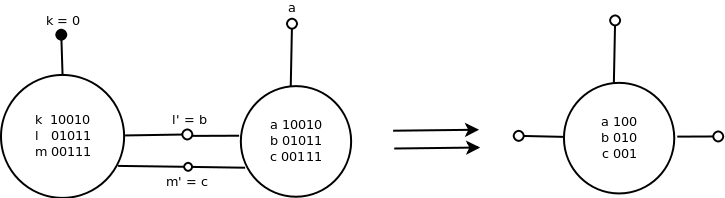
\includegraphics[width=0.9\textwidth]{3_2to3.png}
\caption{Сведение $\pi_5^3$ к $\pi_{symm}^3$ }
\label{fig:3_2to3}
\end{figure}

\begin{figure}[htb]
 \centering
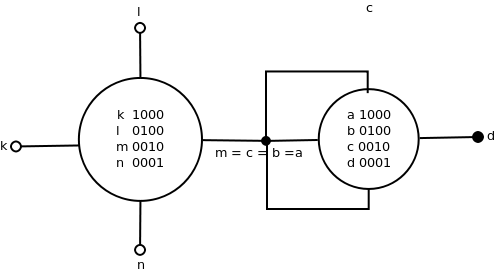
\includegraphics[width=0.6\textwidth]{4to3.png}
\caption{Сведение $\pi_{symm}^4$ к $\pi_{symm}^3$ }
\label{fig:4to3}
\end{figure}

\begin{figure}[htb]
 \centering
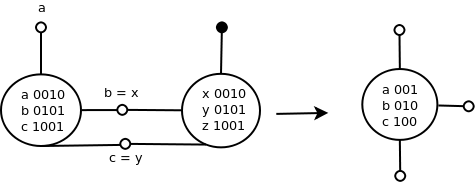
\includegraphics[width=0.7\textwidth]{sch4.png}
\caption{Сведение шефферового предиката с 4 кортежами к $\pi_{symm}^3$ }
\label{fig:sheff4tosheff3}
\end{figure}

\begin{figure}[htb]
 \centering
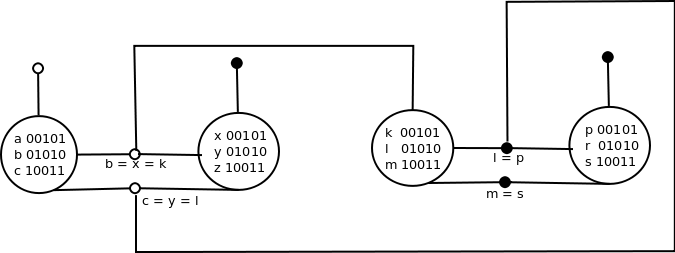
\includegraphics[width=1.0\textwidth]{sch5.png}
\caption{Сведение шефферового предиката с 5 кортежами к $\pi_{symm}^3$ }
\label{fig:sheff5tosheff3}
\end{figure}

%\begin{figure}[htb]
%\centering
%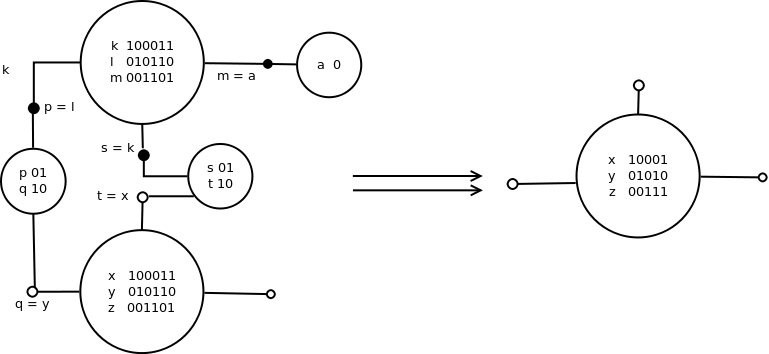
\includegraphics[width=1.0\textwidth]{3_3to3_2.png}
%\caption{Сведение $\pi_{symm+3}^3$ к $\pi_{symm+2}^3$}
%\label{fig:3_3to3_2}
%\end{figure}

%\begin{figure}[htb]
%\centering
%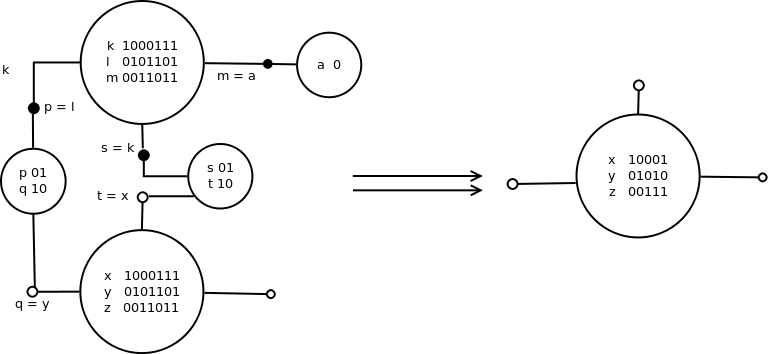
\includegraphics[width=1.0\textwidth]{3_4to3_2.png}
%\caption{Сведение $\pi_{symm+4}^3$ к $\pi_{symm+2}$}
%\label{fig:3_4to3_2}
%\end{figure}

\begin{figure}[htb]
\centering
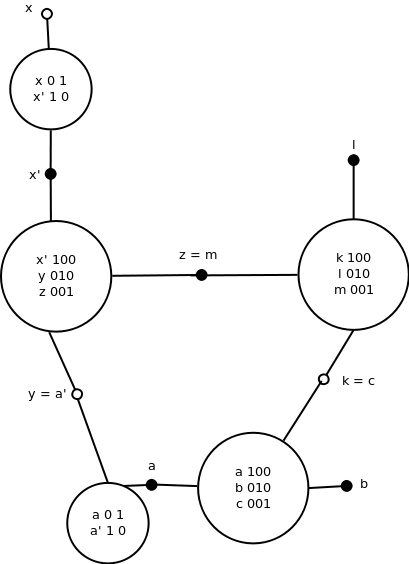
\includegraphics[width=0.6\textwidth]{min_and.png}
\caption{Схема для $\pi_{and}, \Pi_{and} = \{ (000), (010), (100), (111) \}$}
\label{fig:and}
\end{figure}

\begin{figure}[htb]
\centering
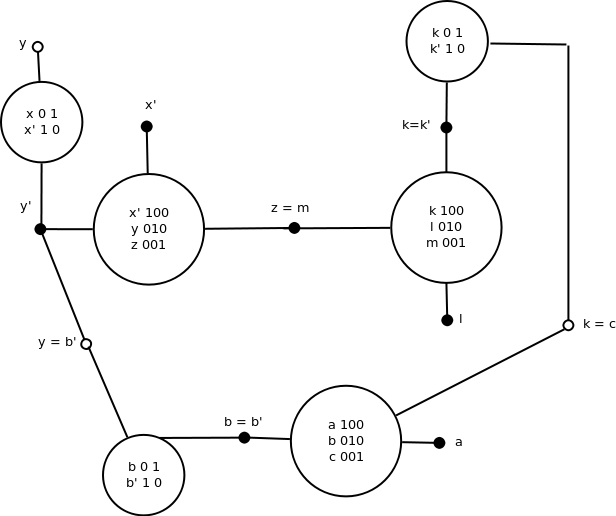
\includegraphics[width=0.9\textwidth]{min_or.png}
\caption{Схема для $\pi_{or}, \Pi_{or} = \{ (000), (011), (101), (111) \}$}
\label{fig:or}
\end{figure}

\clearpage
\section{Заключение}
\subsubsection*{Основные результаты}

\begin{itemize}
\item Исследован вопрос о полноте в классе планарных предикатных схем и установлено, что 
критерий полноты для класса планарных предикатных схем эквивалентен критерию полноты для обычного
класса предикатных схем. 
\item Приведен и оценен алгоритм преобразования непланарной предикатной схемы в планарную 
в произвольном полном базисе. 
\item
В ходе доказательства лемм были уточнены характеристики класса SM, что 
позволяет, например, упростить проверку принадлежности произвольного предиката $\pi$ данному классу. 
Так, было показано, что все предикаты $\pi \notin SM$ имеют в качестве набора допустимых значений расширение симметричного
предиката, причем каждый предикат $\pi(x_1, \dots, x_n) \notin SM$ можно свести к предикату $\pi'(x_1, x_2, x_3)$, 
для которого достаточно проверить лишь сохранение медианы 3 переменных.
\end{itemize}

\subsubsection*{Возможные направления дальнейших исследований}

В \ref{Theo2} был приведен алгоритм планарного сведения произвольного полного базиса к $\pi_{symm}^3$.
Однако за рамками данной работы остался вопрос о способе планарного синтеза схем, реализующих предикат 
с заданной характеристической функцией, например, в том же фиксированном базисе $\pi_{symm}^3$. 
Это исследование стоит поделить на две части, а именно: 
метод синтеза схем, реализующих произвольный предикат от 3 переменных, и метод синтеза схем, реализующих предикаты
большего числа переменных. Данное разбиение на подзадачи придется произвести в силу леммы \ref{susch_lemma} 
о невозможности получения 
существенного предиката от $(n+1)$ переменной применением операции конъюнкции существенных предикатов от $n$ переменных.

% Список цитируемой литературы
\clearpage
\thebibliography{99}
\RBibitem{Shu09}
    \by М.~С.~Шуплецов
    \paper Оценки высокой степени точности для сложности предикатных схем в~некоторых базисах
    \inbook Физико-математические науки
    \serial Уч\"eн. зап. Казан. гос. ун-та. Сер. Физ.-матем. науки
    \yr 2009
    \vol 151
    \issue 2
    \pages 173--184
    \publ Изд-во Казанского ун-та
    \publaddr Казань
    \mathnet{http://mi.mathnet.ru/uzku760}

\bibitem{Shu11}
Методы синтеза и оценки сложности схем, построенных из элементов предикатного типа : 
диссертация на соискание степени кандидата физико-математических наук : 01.01.09 / Шуплецов Михаил Сергеевич; 
[Место защиты: Моск. гос. ун-т им. М.В. Ломоносова] - Москва, 2011 - Количество страниц: 114 с.

\bibitem{CSP10} F. Rossi, P. van Beek and T. Walsh (eds.) Handbook of Constraint Programming, Elsevier, 2010, ISBN 9780444527264.

\bibitem{Bodnar4uk_f}
Боднарчук В. Г., Калужнин Л. А., Котов В. Н., Ромов Б. А. Теория
Галуа для алгебр Поста // Кибернетика. 1969. No 3. C. 1–10; No5. С. 1–9.

\bibitem{graph_first}
Ложкин С. А., Шуплецов М. С. Асимптотические оценки высокой сте-
пени точности для сложности предикатных схем из одного класса //
Материалы XVI Международной школы-семинара 
``Синтез и сложность управляющих систем''(Санкт-Петербург, 26-30 июня 2006 г.). М.:
Изд-во механико-математического факультета МГУ, 2006. С. 72–77.

\bibitem{gt}

Васин А. А., Морозов В. В. Теория игр и модели математической эко-
номики. М.: МАКС Пресс, 2005. 272 с.

\bibitem{mas}
Ferber, Jacques (1999). Multi-Agent Systems: An Introduction to Artificial Intelligence. Addison-Wesley.
ISBN 0-201-36048-9.

\bibitem{yabl_planar}
C.В. Яблонский ``Введение в дискретную математику'' М., Наука, 1988 г

\bibitem{ml}
M. Davis, G. Logemann, and D. Loveland, A Machine Program for Theorem-Proving,
Communications of the ACM, vol. 5, no. 7, pp. 394–397, 1962.

\bibitem{Shaeffer78} Schaefer, Thomas J. (1978). 
``The Complexity of Satisfiability Problems''. STOC 1978. pp. 216–226. doi:10.1145/800133.804350.

\bibitem{Zarank54} Zarankiewicz, K. ``On a Problem of P. Turán Concerning Graphs.'' Fund. Math. 41, 137-145, 1954. 

\bibitem{Prosc89} Arnborg, S.; Proskurowski, A. (1989), 
``Linear time algorithms for NP-hard problems restricted to partial k-trees'',
Discrete Applied Mathematics 23 (1): 11–24, doi:10.1016/0166-218X(89)90031-0.

\bibitem{Gott10} 
Georg Gottlob, Reinhard Pichler, and Fang Wei, 
Bounded treewidth as a key to tractability of knowledge representation and reasoning. 
Artif. Intell. 174, 1 (January 2010), 105-132. 

\bibitem{Diestel00}
Diestel, Reinhard (2000), Graph Theory, Graduate Texts in Mathematics, 
173, Springer-Verlag, ISBN 0-387-98976-5.

\bibitem{Boedlander96}
H. L. Bodlaender, A linear-time algorithm for finding 
tree-decompositions of small
treewidth, SIAM J. Comput. 25 (1996), 1305–1317

\bibitem{Marchenkov}
Марченков С. С. Предполнота замкнутых классов в $P_k$ : предикатный
подход // Математические вопросы кибернетики. Вып. 6. М.: Наука.
Физматлит, 1996. С. 117–132.

\bibitem{Zhuk}
Д.Н. Жук. Решетка замкнутых классов самодвойственных функций трехзначной логики. Издательство МГУ Москва, 2011

\bibitem{Shannon}
Shannon C. E. A symbolic analysis of relay and switching circuits // Trans.
AIEE 57. 1938. P. 713–723.

\bibitem{Shannon2}
Shannon C. E. The synthethis of two-terminal switching circuits // Bell
Syst. Techn. J. 1949. V. 28. N 1. P. 59–98.

\endthebibliography
\end{document}
